\section{Architecture du systéme}
\noindent
Il est indispensable à la conception de tout systéme informatique de choisir le modèle d'architecture adéquat et pourra assurer le bon fonctionnement, une meilleure performance, ainsi que la scalabilité, la fiabilité est trés importante, la productivité du développement. \\
C'est pour cette raison, qu'on a opté pour l'architecture MVC avec des microservices (Modèle, Vue, Contrôleur, Modèle IA, et Elasticsearch) comme l'architecture globale du projet, et le modèle << Clean Architecture >>, dans le backend, qui seront trés pratiques pour gérer les intéractions entre les différents composants de notre application. Nous décrirons ces architectures dans les prochaines sections.

\subsection{Architecture "MVC Avec Microservices"}
\noindent
Le modèle MVC permet de bien organiser son code source. Il va nous aider à savoir quels fichiers créer, mais surtout à définir leur rôle. Le but de MVC est justement de séparer la logique du code en trois parties que l'on retrouve dans des fichiers distincts.

\noindent
{\small\textbf{\textit{Modèle}}}\mbox{}\\
Cette partie gère ce qu'on appelle la logique métier de notre site. Elle comprend notamment la gestion des données qui sont stockées, et aussi le code qui prend des décisions autour de ces données. Son objectif est de fournir une interface d'action la plus simple possible au contrôleur. On y trouve donc entre autres des algorithmes complexes et des requêtes SQL, et Elasticsearch dans notre cas.

\noindent
{\small\textbf{\textit{Vue}}}\mbox{}\\
Cette partie se concentre sur l'affichage. Elle ne fait presque aucun calcul et se contente de récupérer des variables pour savoir ce qu'elle doit afficher. On y trouve essentiellement du code HTML mais aussi quelques boucles et conditions Javascript très simples, pour afficher par exemple une liste de messages. Il est développé avec React et Typescript.

\noindent
{\small\textbf{\textit{Contrôleur}}}\mbox{}\\
Cette partie gère les échanges avec l'utilisateur. C'est en quelque sorte l'intermédiaire entre l'utilisateur, le modèle et la vue. Le contrôleur va recevoir des requêtes de l'utilisateur. Pour chacune, il va demander au modèle d'effectuer certaines actions (demander les produits en fonction d'un mot-clé de recherche) et de lui renvoyer les résultats (la liste des produits). Puis il va adapter ce résultat et le donner à la vue. Enfin, il va renvoyer la nouvelle page HTML, générée par la vue, à l'utilisateur. Il est implémenté avec ASP .NET Core et C\# et utilise des requêtes SQL et Elasticsearch pour manipuler les données.

\noindent
{\small\textbf{\textit{Modèle IA}}}\mbox{}\\
Notre modèle IA a une et une seule responsabilité, qui est de faire l'encodage de la requête de l'utilisateur qui est envoyé au contrôleur et retourner le résultat encodé.

\noindent
{\small\textbf{\textit{Elasticseach}}}\mbox{}\\
Elasticsearch agit comme notre base de données de recherche de vecteurs qui contient notre index de produits contenant 2 colonnes de vecteurs recherchables à l'aide du vecteur codé renvoyé par le modèle AI.

\newpage
\noindent
La figure ~\ref{fig:mvc} schématise le rôle de chacun de ces éléments.
\begin{figure}[H]
\centering
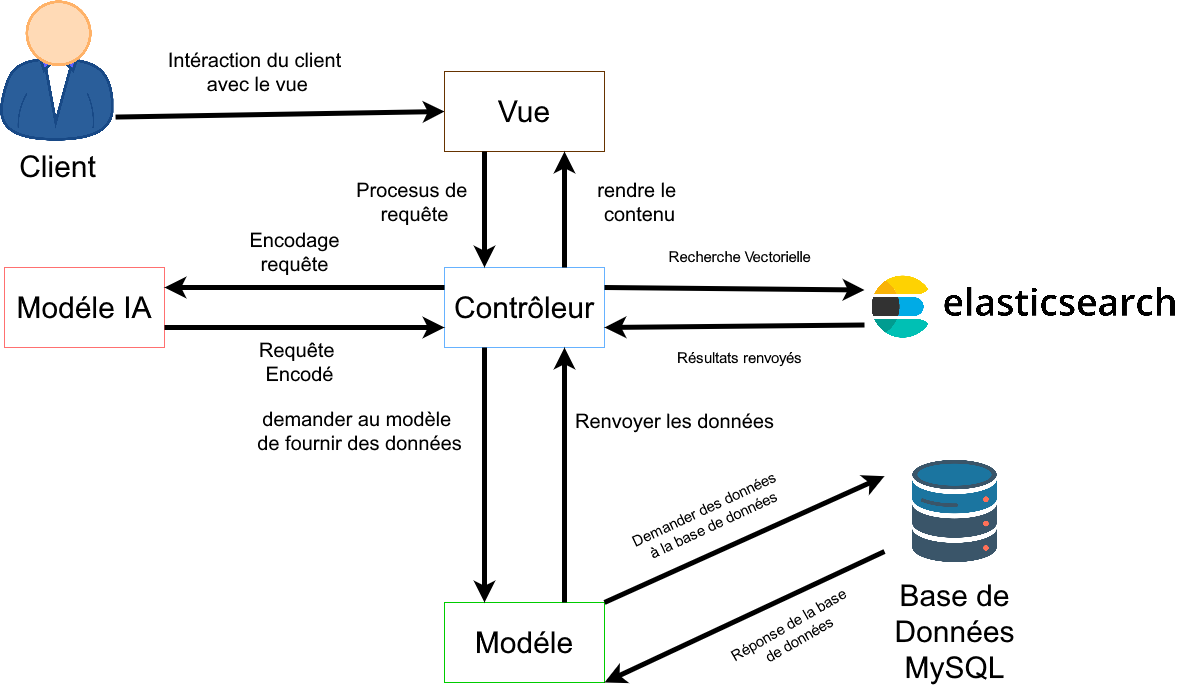
\includegraphics[width=1\textwidth]{logos/mvcavecservice.png}
\caption{L'architecture MVC avec microservices}
\label{fig:mvc}
\end{figure}

\noindent
Il est important de bien comprendre comment ces éléments s'agencent et communiquent entre eux. La figure ~\ref{fig:mvcechange} montre cette communication.

\begin{figure}[H]
\centering
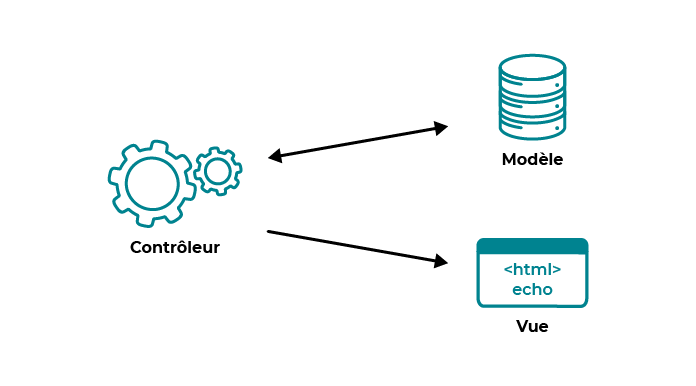
\includegraphics[width=1\textwidth]{logos/mvcechange.png}
\caption{Échange d'informations entre les éléments MVC}
\label{fig:mvcechange}
\end{figure}

\subsection{Architecture "Clean Architecture"}
\noindent
"Clean Architecture" est un modèle architectural introduit par Robert C. Martin, également connu sous le nom d'Oncle Bob. Il favorise une séparation claire des préoccupations en divisant l'application en couches concentriques, chaque couche ayant ses responsabilités et ses dépendances. Le principe fondamental derrière l'architecture propre est la règle de dépendance, qui stipule que les dépendances doivent toujours pointer vers l'intérieur vers les couches les plus stables et abstraites, plutôt que vers l'extérieur vers des couches plus concrètes et volatiles. 

\noindent
Cette architecture se compose généralement des couches suivantes: \\

\begin{itemize}
    \small\item \textbf{La couche Présentation: } Cette couche est responsable de la gestion des interactions des utilisateurs et de la fourniture des données à l'interface utilisateur. Dans notre context d'une API Web .NET Core, cette couche comprend les contrôleurs et autres composants qui gèrent les requêtes et les réponses HTTP.

    \small\item \textbf{La couche Application: } La couche Application contient la logique métier et les cas d’utilisation de l’application. Il agit comme intermédiaire entre la couche présentation et la couche domaine. Cette couche est indépendante de tout problème spécifique d’interface utilisateur ou d’infrastructure.
    \small\item \textbf{La couche Domain: } La couche Domain représente le noyau de l’application, encapsulant les règles métier, les entités, les interfaces (Orienté Objet) des repositories des bases de donnés et la logique spécifique au domaine. Il doit être indépendant de la technologie et ne continent aucune dépendance vis-à-vis de frameworks ou de bibliothèques externes.

    \small\item \textbf{La couche Infrastructure: } La couche infrastructure traite des problèmes externes tels que les bases de données, les services externes et les frameworks. Elle contient des implémentations d'interfaces définies dans la couche application et interagit avec des ressources externes.
\end{itemize}

\noindent
La figure Figure~\ref{fig:architecture} reprèsente les couches de << Clean Architecture >>

\begin{figure}[H]
\centering
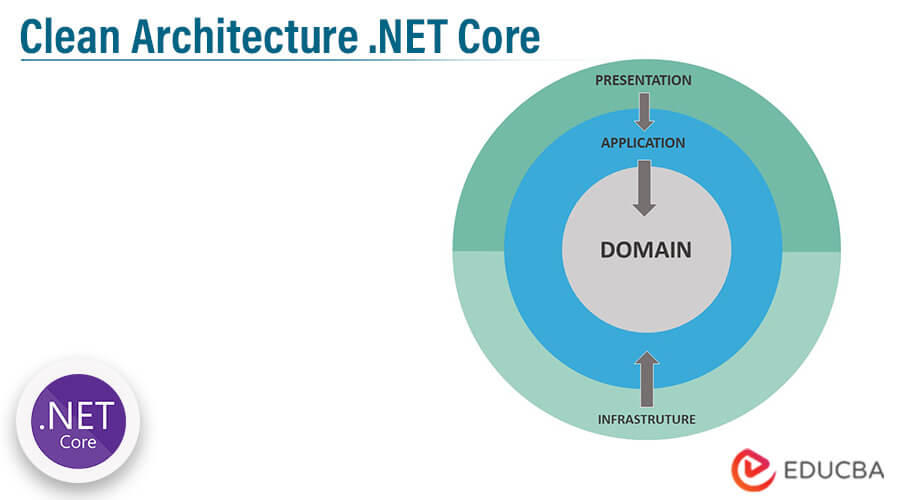
\includegraphics[width=1\textwidth]{logos/clean_architecture.png}
\caption{Architecture "Clean Architecture" dans ASP. NET Core}
\label{fig:architecture}
\end{figure}

\noindent
Les avantages de l’utilisation de  << Clean Architecture >> :

\begin{itemize}[label={---}]
    \item \small\textbf{Vitesse d'implémentation: } La mise en œuvre immédiate vous permet d'implémenter cette architecture avec n'importe quel langage de programmation.

    \item \small\textbf{Les couches de Domain et Application comme noyau du système}: Les couches Domain et Application sont toujours au centre de la conception et sont connues comme le cœur du système, c'est pourquoi le cœur du système ne dépend pas de systèmes externes. 

    \item \small\textbf{Indépendence des systémes externes: } Cette architecture permet de changer de système externe sans affecter le cœur du système.

    \item \small\textbf{Testabilité améliorée du code: } Dans un environnement qui dépends hautement des tests(unitaires et d'intégration), vous pouvez tester votre code rapidement et facilement.    

    \item \small\textbf{Création de produits scalables, robustes et de hautes qualité: } Vous pouvez vitement créer un systéme bien performant, organisé, testable, scalable, et robuste.
\end{itemize}
\noindent